
\documentclass[letterpaper,twocolumn,10pt]{article}
\usepackage{usenix,epsfig,endnotes}

\usepackage{color}
\usepackage{psfrag}
\usepackage{subfigure}
\usepackage{booktabs}
%\usepackage{float}
\usepackage{url}
\usepackage{path}
\usepackage{caption}
\usepackage{courier}
\usepackage{listings}
\usepackage{pifont}
\usepackage{graphicx}
\usepackage{minted}




%don't want date printed
\date{}

%% disable the splitting of footnotes
\interfootnotelinepenalty=10000

%% source code styles
\lstset{
	basicstyle=\footnotesize\ttfamily,
	extendedchars=true,
	breaklines=true,
	frame=lines
}

%% table style
\renewcommand{\arraystretch}{1.1}

\begin{document}

% key words
\newcommand{\cb}{CloudBrowser}
\newcommand{\js}{JavaScript}
\newcommand{\nodejs}{Node.js}
\newcommand{\appins}{App Instance}
\newcommand{\citemain}{~\cite{mcdaniel2012cloudbrowser}}

% section for figs
% maybe put this in a figure.tex
\newcommand{\architectureoverview}{
    \begin{figure*}[ht]
    \centering
    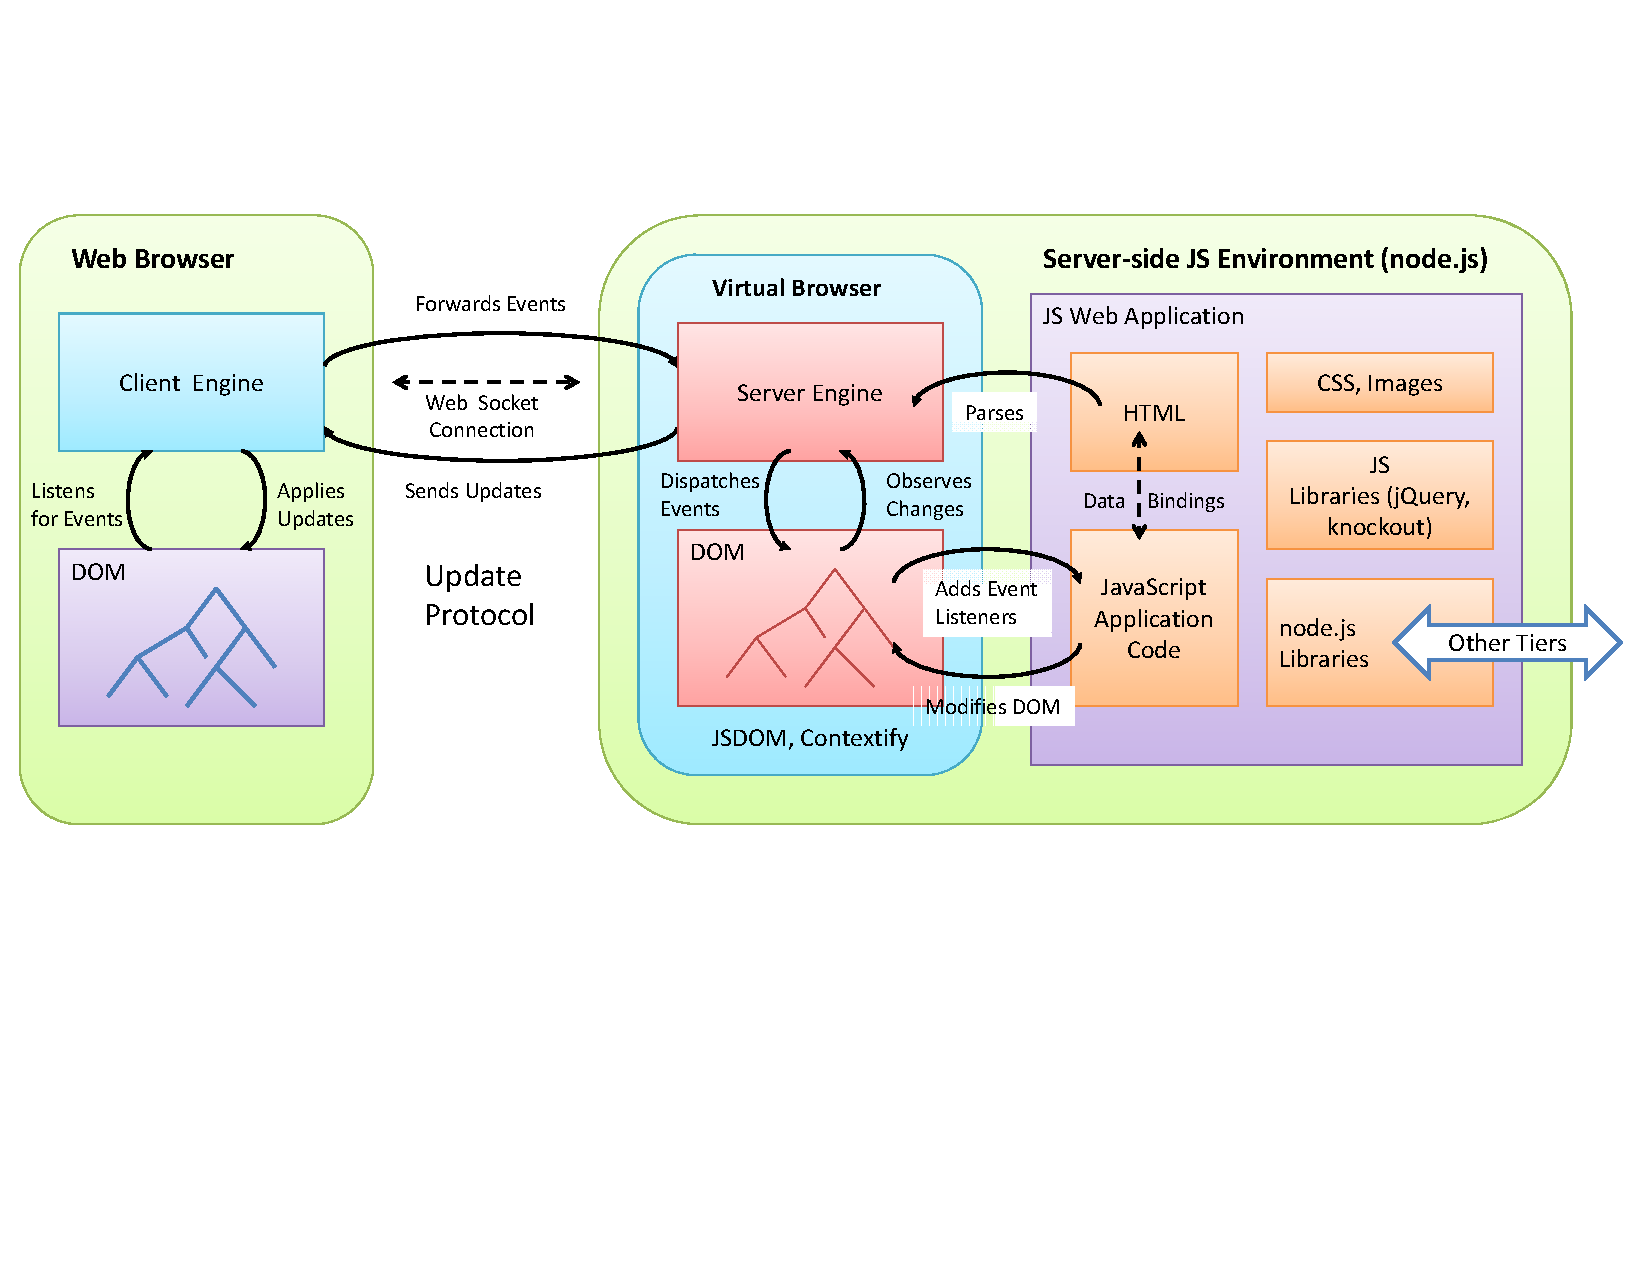
\includegraphics[width=\textwidth]{figs/architecture_overview}
    \caption{Single Process \cb{} Architecture Overview}
    \label{fig:cb1arch}
    \end{figure*}
}

\newcommand{\newarchitectureoverview}{
    \begin{figure*}[ht]
    \centering
    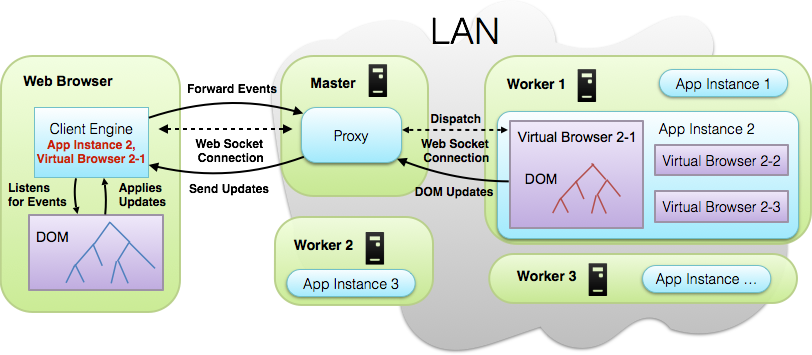
\includegraphics[width=\textwidth]{figs/new_architecture_overview}
    \caption{Multiprocess Process \cb{} Architecture Overview}
    \label{fig:cb2arch}
    \end{figure*}
}

\newcommand{\requestdispatchdiagram}{
    \begin{figure}[ht]
    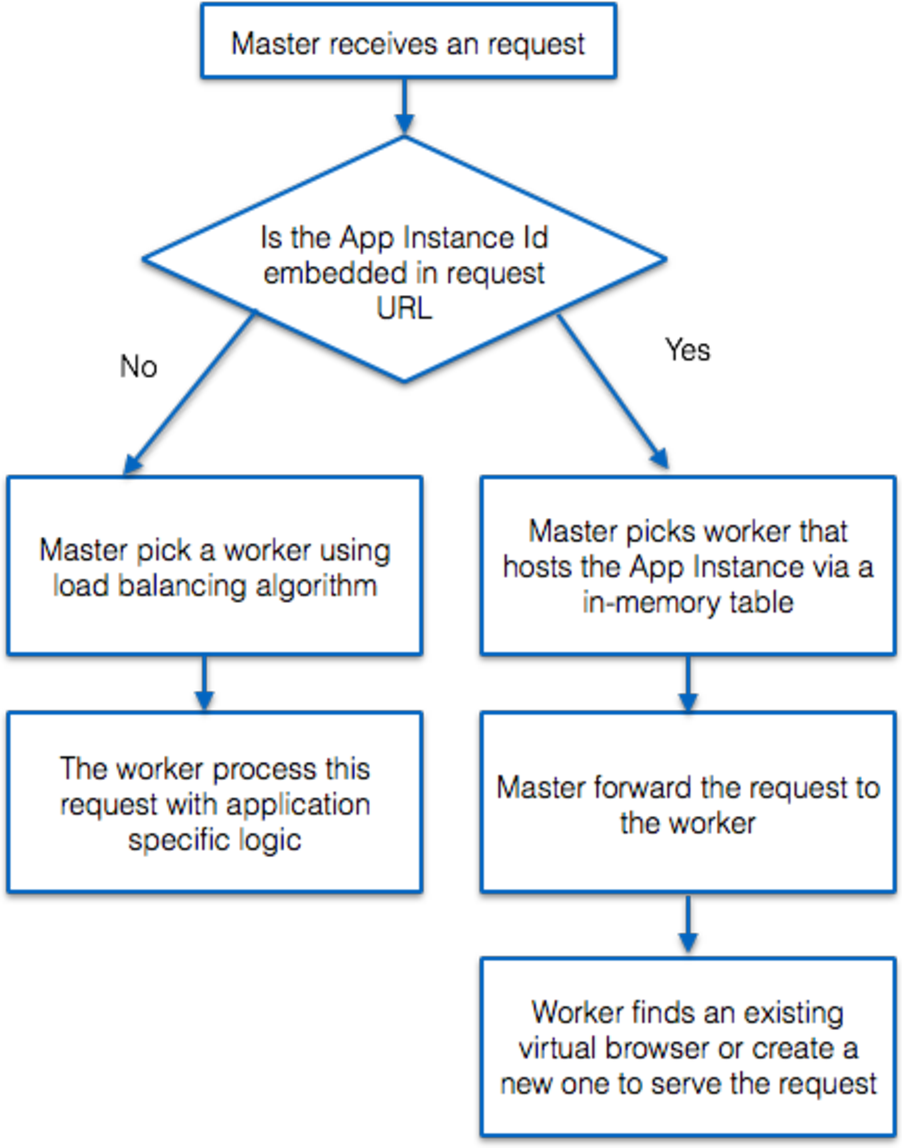
\includegraphics[width=0.4\textwidth]{figs/request_dispatch}
    \caption{Request Dispatch Diagram}
    \label{fig:dispatch}
    \end{figure}
}

\newcommand{\appinstancefig}{
    \begin{figure}[ht]
    \centering
    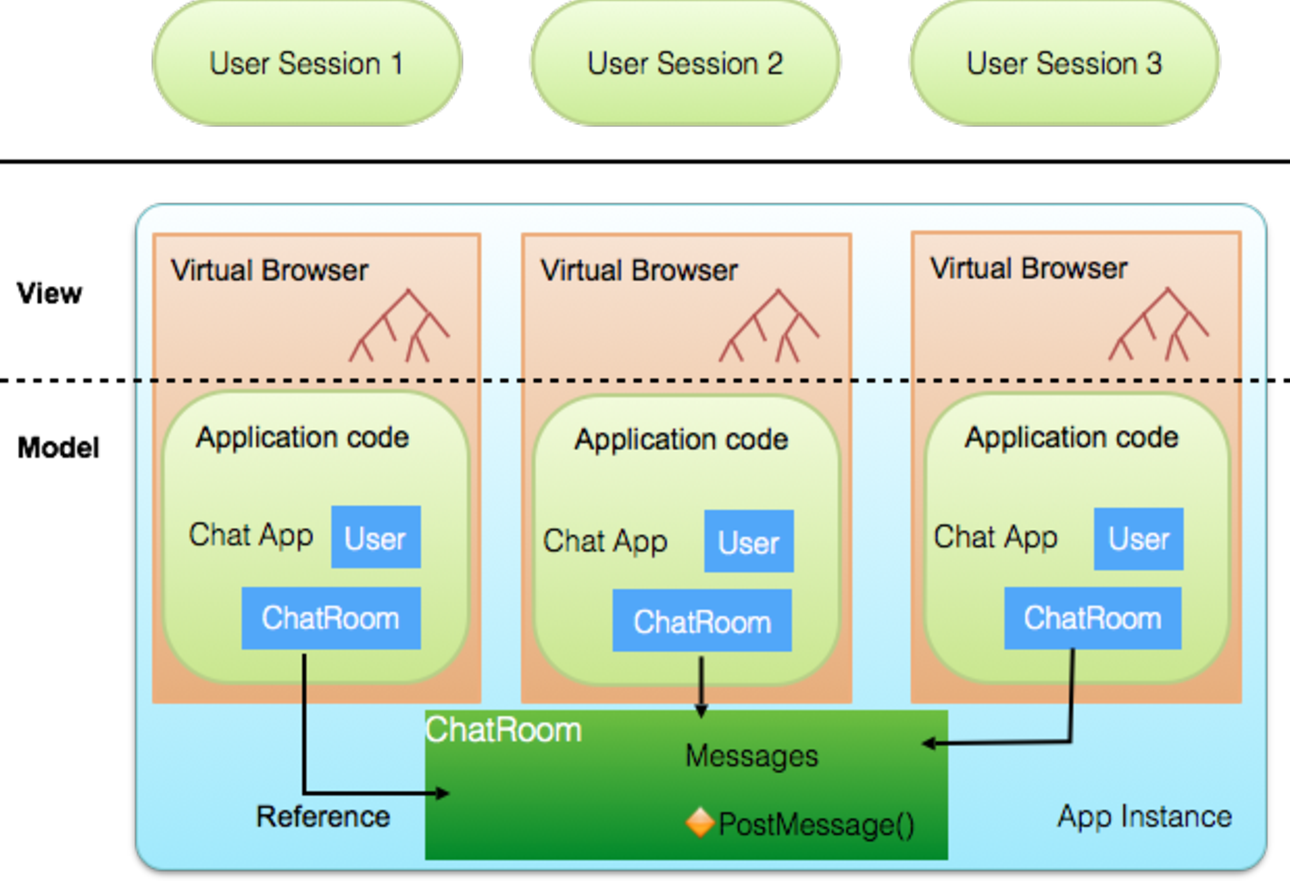
\includegraphics[width=0.5\textwidth]{figs/appInstance}
    \caption{Detailed view of an App Instance}
    \label{fig:appinstance}
    \end{figure}
}


\newcommand{\multiappservers}{
    \begin{figure}[ht]
    \centering
    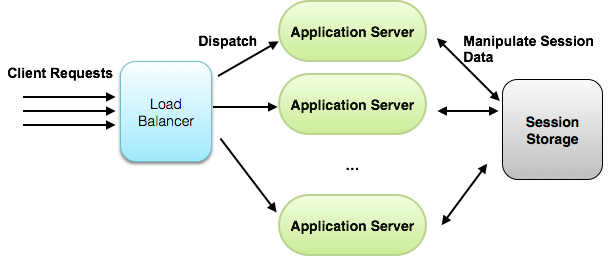
\includegraphics[width=0.5\textwidth]{figs/multiple_app_servers}
    \caption{Scaling out a web application}
    \label{fig:multiappservers}
    \end{figure}
}


\newcommand{\clickthroughput}{
    \begin{figure}[ht]
    \centering
    \includegraphics[width=0.5\textwidth]{gnuplot/click_throughput}
    \caption{Throughput of click application.}
    \label{fig:clickthroughput}
    \end{figure}
}


\newcommand{\clicklatency}{
    \begin{figure}[ht]
    \centering
    \includegraphics[width=0.5\textwidth]{gnuplot/click_latency}
    \caption{Latency of click application.}
    \label{fig:clicklatency}
    \end{figure}
}


\newcommand{\clickwaitthroughput}{
    \begin{figure}[ht]
    \centering
    \includegraphics[width=0.5\textwidth]{gnuplot/click_wait_throughput}
    \caption{Throughput of click application, after introducing artificial delay.}
    \label{fig:clickwaitthroughput}
    \end{figure}
}


\newcommand{\clickwaitlatency}{
    \begin{figure}[ht]
    \centering
    \includegraphics[width=0.5\textwidth]{gnuplot/click_wait_latency}
    \caption{Latency of click application, after introducing artificial delay.}
    \label{fig:clickwaitlatency}
    \end{figure}
}



\newcommand{\angularchatlatency}{
    \begin{figure}[ht]
    \centering
    \includegraphics[width=0.5\textwidth]{gnuplot/angularchat_latency}
    \caption{Latency of chat application with Angular.js.}
    \label{fig:angularchatlatency}
    \end{figure}
}


\newcommand{\jquerychatlatency}{
    \begin{figure}[ht]
    \centering
    \includegraphics[width=0.5\textwidth]{gnuplot/jquerychat_latency}
    \caption{Latency of chat application with JQuery.}
    \label{fig:jquerychatlatency}
    \end{figure}
}

\title{\Large \bf Multiprocessor \cb}

\author{Xiaozhong Pan  \qquad  Godmar Back\\
Department of Computer Science\\ 
Virginia Tech\\
\url{bladepan@cs.vt.edu} \qquad  \url{gback@cs.vt.edu}
}




\maketitle
\thispagestyle{empty}

%% remove newpage here
\begin{abstract}

% Usenix style
% \subsection*{Abstract}
% todo more description about cb
Designing modern web applications involves a wide spectrum of
choices when it comes to deciding where the different tiers of
application and framework code that constitute these distributed
applications should be placed.  These system design choices affect 
programmer productivity, ease of deployment, security, and performance, 
particularly with respect to latency and scalability.

In this paper, we propose and evaluate an extreme design choice
in which not only all application logic executes server-side, but
most presentation logic as well.  The client browser is reduced to
a rendering and I/O engine, similar to a ``thin client'' or ``dumb 
terminal.''

We have developed CloudBrowser 2.0, a system that implements this
distribution model using a scalable multiprocess approach.  
In this paper, we perform an evaluation of the benefits and costs of 
this approach when compared to both more traditional approaches as well 
as emerging alternatives.  We focus on 
programmability and systems aspects including performance and latency. 

\end{abstract}


\newpage
\section{Introduction}
\label{sec:intro}

% backgroud, motivation, design choices, architecture , experiments(goals, etc.)
Before AJAX~\cite{garrett2005ajax} became pervasive, most web site works like this:
the user sends a request to the web server through submitting a form or clicking a link on a web page,
then the server processes this request and responds a new HTML document.
In this model, the application logic resides mainly on server side, the client side is mostly
plain HTML document.
The problem about this form/link based model is that it is hard
to create responsive and rich user experience because the whole user interface
is wiped out and re-rendered every time user sends a request.

AJAX is an approach that uses javascript to send requests to server
and partially update the HTML document without page refresh.
It is capable of delivering a better performance and native application like user experience.
In this model, developers have to write client javascript code to handle server client communication
and rendering logic. 


\cb{} is a server-centric framework designed to simplify the development of AJAX web applications.
Developer's code is running in a server side virtual browser and the user's browser is just
a dumb display device which synchronizes with the virtual browser.
In \cb{}, developers use nothing but HTML, css and javascript to construct the UI logic just like
any traditional AJAX application.
In the place where traditional AJAX applications call a server side API through HTTP,
developers could call a server side method directly.
The synchronization between the virtual browser and the actual browser is 
handled by the framework under the hood.
\cb{} also naturally preserves UI state upon page refreshes
because all the UI state is kept in the server side.



%Comparing to other server-centric frameworks, 
%\cb{} could reuse most of existing client code because it does not require an extra markup language
%and its sole programming language is javascript.


The original \cb{}'s architecture is restricted to a single process.
It cannot benefit from multiple processors and provides no isolation between virtual browsers.
The stateful nature of \cb{} makes it hard to support multiple process, 
but we think it is a effort worth taking for it would not only boost \cb{}'s capacity
but also shed some light on how to scale nodejs applications in general.





\section{Motivation}
\label{sec:moti}

We motivates our approach to help developers to write scalable continuous web applications.
People use multiple devices to access web applications all the time, 
preserving the view state of the web application and presenting
users synchronized view on all their devices enhances user experience.
They could use web applications seamlessly on all their devices
without the hassle of manually restoring to the state where they left.
Moreover, as operating systems like IOS and MACOS introduces features
like continuity to synchronize states of native applications among multiple
devices, users would expect web applications to work like those native counterparts.
In the other way around, native application developers could use \cb{} to 
implement continuous native applications based on HTML.

Web application owners constantly need to increase the capacity of web applications due
to the increase of user loads or the applications themselves demand more resource
as they evolve.
The architecture solutions to scale a web system can be categorized into 
scale-up and scale-out~\cite{cardellini2002state}.
Scale-up is to increase the performance of a single server,
it can be achieved by upgrading the server hardware or optimizing software.
Scale-out is to employ more servers and distribute load among all servers.
In this paper, we will only discuss scale-out solutions and scale-up in
a sense that software could leverage the power of multiple processors.
As other solutions such as increase memory capacity, optimizing operating system,
tuning application software is applicable to all web frameworks.
As Fig.~\ref{fig:webscaleout} shows, 
a scale out web system architecture consists a load balancer and multiple
application servers.
The load balancer distribute requests from clients to the application servers,
application servers host business logic and generate content for client requests.
Here the load balancer could be one or multiple special purpose hardware or reverse 
proxy software like nginx or apache HTTP server deployed on general purpose 
machines, it could also be a conceptual part that handles distribution logic:
for example the web system owner could register IP addresses of all the application
servers to DNS server, and rely on the client browser to distribute its requests to
all the IP addresses.

A common strategy for load balancer is to distribute requests in a content-blind manner,
for example, it pick an application server randomly or in a round robin fashion.
The downside of this approach is that 
for every request the application server needs to restore the application state
as it could receive requests from any user.
For example, the application server need to 
fetch the user name from database when the user's request hit it for the first time,
and this db access is duplicated when the user's requests 
are routed to other servers.

To reduce these redundant work, some web system owners adopt
session affinity distribution.
This approach distributes requests from a user to the same application server,
so the application server needs only create application state once.
In this approach, the load balancer is often implemented by reverse proxy software
like nginx.


In \cb{}, a virtual browser keeps the view 
\cb{} is session-aware by design because 
the user's requests are handled by virtual browsers,
a virtual browser contains the application state and view state.
We will discuss how to distribute virtual browsers among multiple servers
 in detail in section~\ref{sec:implementation}.

On top of virtual browser, 
\cb{} has a level of abstraction called \appins{} that is helpful
to build collaborative applications.
An \appins{} is a group of virtual browsers that are guaranteed to be placed
in the same \cb{} process.
The virtual browsers from the same \appins{} share a user defined \appins{} object.
The developer could use a \appins{} object to describe an entity that 
could be accessed by multiple users, 
then create virtual browser under that \appins{} as user's views of this shared entity.
For example, the application could use an \appins{} object as a shared document and 
define various properties and methods on that object.
Whenever a user want to edit that document, the application
creates a virtual browser under that \appins{},
the user specific application state like user name and editor settings 
could be stored in variables inside his virtual browser.
The application could use the \appins{} object directly to render the document for every user, 
and each user can have his own view of the editor.

Current web frameworks do not have such clear construct to define application state.
One option for the developer is to rely on session objects provided by frameworks.
The application developer needs to configure the persistence  of session objects 
and make sure the configuration works with the load distribution scheme.
For example, in J2EE the session objects could be configured to be stored in memory or
high available database~\cite{j2eedoc}; 
PHP developers need to specify a session save handler to store session objects 
in database~\cite{phpdoc}.
By default, these frameworks store session objects in memory or in local file system.
If the developer adopts a content-blind load balancer, 
he should also configure the session objects to use database or other
synchronization mechanism.
If the developer uses a session affinity load balancer,
he should configure the session objects to be stored in local memory.
Another option is to implement his own way of handling application state.
The developer also needs to make sure his implementation works with
his load balancer.

\cb{} does not have the concept of session,

% That means the applications will not scale if not configured properly.
% Second, the load distribution scheme and 
% Even everything is correctly configured, 
% the developer also needs to write boilerplate code to retrieve objects from the
% session object to restore application state for every request.


% Also, \cb{} makes it clear how the work load is distributed.


\webscaleout{}
\chapter{Implementation}
\label{ch:impl}
\markright{Implementation}

This chapter first discusses the overview of the multi-process architecture of \cbtwo.
Then we discuss how client requests are dispatched and how load balancing is implemented.
After that we discuss the implementation of different \cbtwo processes and how they interact
with each other.
In the end we discuss how \cb applications access the framework internal objects.

%Since virtual browsers occupy most of the system resources, the new
%distributed design spread the virtual browsers to multiple processes
%to improve the system's scalability.


As shown in Figure~\ref{fig:cb2arch}, \cbtwo consists of a
single master process, multiple reverse proxies, and multiple worker
processes. All processes communicate via nodermi, which in turn uses standard TCP/IP 
sockets in its transport layer, so they can
be located on a shared-memory multiprocessor machine or on different machines in a cluster. 
Worker processes host application instances and virtual browsers. The master process is responsible for
the request dispatch logic which decides how to distribute the client load to
workers. The actual dispatching is implemented by the reverse proxies, which
forward users' requests to workers and copy workers' responses back to users.
All reverse proxy processes are bound to the socket that accepts client
requests, allowing the OS to distribute pending client connections in a round-
robin fashion.
The reverse proxy can relay both HTTP requests/responses as
well as the bidirectional WebSocket protocol (see Section~\ref{sec:nodepackage}).
Once the client has established a WebSocket connection with
the server side, the majority of traffic will be WebSocket
messages for which there is relatively little per-message overhead.

\newarchitectureoverview{}


% The master process is a single point of failure,
% but it is light weight and does less computation,
% so it is less likely to fail in practice.

\section{Request Dispatch}
\label{sec:reqdis}

When a request is being dispatched, the reverse proxy uses information
contained in the request URL to make an appropriate forwarding decision. 
The system exposes three types of URLs for the users to access \cb applications.
The formats of these URLs are as follows:

\begin{description}

\item[Application URL] \label{itm:appurl} \hfill \\
\url{http://example.com/[app]}. \\
\code{[app]} represents an application's mount point. 
For example, if an application's mount point is
\emph{chat},  then its Application URL is \url{http://example.com/chat}.


\item[\appins{} URL] \label{itm:appinsurl} \hfill \\
\url{http://example.com/[app]/a/[appInstanceId]}. \\
\code{[app\-Instance\-Id]} represents an \appins{}'s id.  For example, if an
\appins{}'s id is \emph{appins1} and its application's mount point is
\emph{chat}, then its \appins{} URL is
\url{http://example.com/chat/a/appins1}.


\item[Browser URL] \label{itm:vburl} \hfill \\
\url{http://example.com/[app]/a/[appInstanceId]/b/[browserId]}. \\
\code{[browser\-Id]} represents a virtual browser's id. For example, if a
virtual browser's id is \emph{browser1} and its \appins{} id is 
 \emph{appins1} and its application's mount point is \emph{chat},
  then the virtual browser's Browser URL is 
  \url{http://example.com/chat/a/appins1/b/browser1}.

\end{description}

% TODO justify why you included /a and /b (for clarity?)

From the user's point of view, the \emph{Application URL} is similar to  the
homepage URL in a traditional web application. For a \emph{singleAppInstance}
or \emph{singleInstancePerUser} application, requesting \emph{Application URL}
redirects the user to the only virtual browser  he can access, the virtual
browser is created automatically if it did exist before the user request. For
a \emph{singleBrowserPerUser} or \emph{multiInstance} application, requesting
\emph{Application URL} redirects the user to the landing page
(Figure~\ref{fig:landingpage})  in which he can navigate to any of his virtual
browsers. The user may prefer use \emph{Application URL}s because it is easy
to remember and he can access his virtual browsers from \emph{Application
URL}s without bookmarking individual virtual browsers' URLs.

\landingpagefig{}


\emph{\appins{} URLs} are used for joining a specific, already created
\appins{}.   For \emph{singleBrowserPerUser} applications where each user can
create only  one virtual browser for a given \appins{}, the system directs the
user to his own virtual browser in the specified \appins{} when handling
\emph{\appins{} URL}.

For \emph{multiInstance} applications, it is the user's responsibility to
decide whether they wish to join an existing virtual browser or create a new
one, the system will lead the user to a landing page to make that decision.
For \emph{singleBrowserPerUser} and \emph{multiInstance} applications, users
can share an \appins{} with others by sharing its \emph{\appins{} URL}.

\appins{} URLs are not meaningful for \emph{singleAppInstance}   and
\emph{singleInstancePerUser} applications because there is only one \appins{}
for a given user.

\emph{Browser URLs} are for connecting to a specific virtual browser. A user
can bookmark a \emph{Browser URL} so he can revisit that specific  virtual
browser in the future. The user can also share a virtual browser with other
people by sharing its \emph{Browser URL}.

As discussed in Section~\ref{sec:deploymodel}, multiple virtual browsers may
share data structures belonging to an \appins{}. \cbtwo colocates every
\appins and its virtual browsers in the same worker process. Once an \appins
has been created in a particular worker process, all future requests to
\emph{\appins{} URL}s and \emph{Browser URL}s for that instance's ID must be
routed to that worker. When the user requests an \emph{Application URL},  the
system needs either allocate  a virtual browser  or redirect the user to a
landing page according to the application's instantiation strategy. Because the
landing page itself is a virtual browser,  the
system always allocates a virtual browser for the  user when handling user's
\emph{Application URL} request. Then the system redirects the user with the
virtual browser's URL.

%Application URL}s, the system need first allocate an \appins{} and virtual
%browser to handle the request according to the instantiation strategy, and then
%redirect the request with the virtual browser's URL.

Although the reverse proxy processes are in charge of the actual forwarding,
the master process keeps track of the forwarding map. Thus,
when a client sends a HTTP request, a reverse proxy process
will accept this HTTP request and ask the master where to dispatch this request. 

If the request URL is a \emph{Browser URL} or \emph{\appins URL}, 
the master extracts \appins id from the URL and returns the associated
worker via a \appins id to worker lookup table.
This lookup table is updated every time an \appins{} is created or removed.
For an \emph{\appins URL} request, the worker will continue to find the associated
virtual browser for the user and send back a redirect with the virtual browser's URL.

If the request URL is an \emph{Application URL}, 
the system's behavior varies according to the application's instantiation strategy.
For example, for a \emph{singleInstancePerUser} application,
the system can either create a new \appins{} for the user if the user does not have an
\appins or use the user's existing \appins{} if otherwise.
The instantiation strategy specific logic is handled by workers, not the master,
because it requires access to authentication information.
Thus, the master can pick any worker using a load
balance algorithm (detailed in Section~\ref{sec:lb}),
and the selected worker will then process the request according
to the instantiation strategy.
After consulting the authentication information, this worker will redirect 
the client to a specific Browser URL.   The virtual browser corresponding
to that URL may be located in another worker process.

When a worker process receives a Browser URL request, it will locate the
corresponding virtual browser and responds with an HTML document that contains
information to bootstrap the client engine. 
The client engine will create a WebSocket connection to establish an RPC channel to
the worker process.
First, the client engine sends a WebSocket handshake request to initiate the
WebSocket connection.
The handshake request URL contains the associated \appins id and virtual browser
id so the master can find the corresponding worker for this request.
After the worker sends back the handshake response, the connection
between the worker and the reverse proxy that performed the handshake, 
as well as the connection between the reverse proxy and the user remains open. 
The reverse proxy will relay all subsequent WebSocket messages
without parsing them and without requiring repeated calls to the master
to obtain forwarding information.

As the client engine renders the client-side view of the page, it may trigger
requests for auxiliary resources such as images or spreadsheets. 
These requests will contain the \appins{} id in the URL, which the master
uses to forward those requests to the appropriate worker.

%If any exception happens, for example, the user sends a Browser URL with no
%corresponding virtual browser in the system, the system will reject the
%request with an error message.

In this design, the reverse proxies ask the master for the dispatch decision
for every HTTP request.  However, HTTP requests are required only when users
reconnect to virtual browsers - most of the actual interaction with a virtual
browser is performed using RPC messages carried over WebSocket connections.
Thus, the overhead of inter-process communication between the reverse proxies and
the master to obtain forwarding information affects only a small portion of the network traffic. 

We also provide an option to embed a reverse proxy instance inside the master process.
If the system is configured with one single embedded reverse proxy,
reverse proxy and master can communicate directly.
However, in this mode, the system can support fewer concurrent users than 
when using multiple reverse proxies.

\section{Load Balancing}
\label{sec:lb}

The load balancing algorithm is invoked in two scenarios:
First, when the user requests an \emph{Application URL},
the master needs to find a worker to handle this request.
Second, it is invoked when the system is about to create an \appins{}.
Although such action can originate in any worker,
the load balancing algorithm is performed by the master.

For other user requests the routing is determined by the \appins{}-to-worker map
so there is no need for load balancing.
In particular, the creation of virtual browsers is not subject to load balancing.
Virtual browsers have to be placed in the same worker that hosts its \appins{}.

We support two load balancing strategies: first, the master can assign the
load to workers in a simple round-robin fashion. However, since \appins{}s may
vary widely in terms of the actual cost they impose on a worker and \appins{}s
can be terminated, the round-robin assignment works well only for cases in 
which resource use is uniformly distributed.
We also implemented a load-based scheme in which
workers periodically report a measure of current load to the master. The
master will select the worker with the lowest load when making load balancing decisions.
We have found the amount of heap memory that is currently in use a good measure
of a worker's momentary load.

In the load-based mode, the master's knowledge of a worker's load is not
always up-to-date as the worker's load can change before the master receives the
next report from the worker. We have found that this can lead to very unbalanced load
distributions. For example, when the system is creating a burst of \appins{}s,
they are all assigned to the same worker that has the lowest load at that
moment and this worker ends up hosting a disproportionate load.  To mitigate
this issue,  after the load balancing algorithm selects a worker, the
algorithm makes a projection of the worker's load after accepting the new
load. The projected value is used as the worker's load value  until the master
sees the worker's next report.  We have found it unnecessary to exactly 
predict the amount of incremental load as long as we do not significantly 
underpredict.  Based on our evaluation, a virtual
browser in a non-trivial application takes about 6M.  The master projects a
worker's load increase by 10M for every new \appins assignment assuming every
\appins will create 1 or 2 virtual browsers.  For most cases, the master
overestimates the actual load increase. It is not a problem because the master
corrects its estimate as soon as it sees the worker's next report. 
% ???
%In our experience, even under bursts of new requests the load distribution among the
%workers does not vary greatly.

\section{Master Implementation}
\label{sec:masterimpl}

This section describes the main modules in the master and how they interact
with worker processes.

\begin{description}
\item[Application Manager] \hfill \\
The Application Manager is responsible for maintaining the state of applications. 
It reads application bundles (discussed in Section~\ref{sec:deploymodel}) and
initializes the data structures used to represent applications.

\item[Worker Manager] \hfill \\
The Worker Manager is responsible for the request dispatch
and the load balancing algorithm.

\item[Reverse Proxy Manager] \hfill \\
The Reverse Proxy Manager starts multiple reverse proxy processes as child
processes of the master and handles the communication between the master and
the reverse proxies.
% the queries are sent from pipe, called ipc channel in node.js
% https://github.com/joyent/node/blob/master/lib/child_process.js
\end{description}

After initialization, the master exposes the \emph{Application Manager} and
\emph{Worker Manager} objects to the workers via nodermi's \code{registerObj} method
(discussed in Chapter~\ref{ch:rmi}).

The \emph{Application Manager} includes methods related to application management,
such as listing applications, creating new applications, removing applications,
etc.  The applications are represented by application objects. An application
object has methods to manage the internal state of an application, which include
methods to change the application's authentication policy, register a new \appins, 
remove an \appins, etc.  Since the \emph{Application Manager} is registered in nodermi,
workers can obtain remote references to it; the application objects returned by its
methods are also automatically represented as nodermi remote references.
The master's Application Manager coordinates with the Application Manager
objects in each worker as described in Section~\ref{sec:worker}.

The \emph{Worker Manager} contains methods for workers to register the URL at which
they can be reached and report their load.  It maintains a table of \appins{} id to
worker URL for dispatching requests.  This table is updated
every time a \appins{} is registered or removed from the \emph{Application
Manager}.

\section{Worker Implementation}
\label{sec:worker}

This section describes the implementation of worker processes.
The key components of a worker process include:

\begin{description}

\item[Application Manager] Manages applications' metadata, application instantiation
logic, local \appins{}s
and local virtual browsers. It provides methods to lookup local \appins{}s and virtual
browsers by ids. It also processes incoming HTTP requests.

Workers pass a reference to the \emph{Application Manager} and application objects to
the master's \emph{Application Manager} via remote method invocation.  The
master uses remote references to these worker
objects to push application-related changes to the  workers.  For instance,
the master calls  a worker's \code{addApplication} method remotely to
push new applications to that worker and remove an application from that worker
by calling the worker's \code{removeApplication} method remotely.

\item[Session Manager] 
Manages HTTP sessions and users' login states. The sessions
are stored in a database server that is accessible for all workers. 
The users' login states are stored in session properties 
as discussed in Section~\ref{sec:auth}.


\item[HTTP Server] Listens for HTTP requests from reverse proxies and dispatches 
    the requests to the \emph{Application Manager}. 

\item[Permission Manager] 
Manages users' permissions to applications, \appins{}s and virtual browsers.
If an application enables authentication, it can call the \emph{Permission
Manager} to grant or revoke access to  \appins{}s and virtual
browsers for specific users. 

The system will reject HTTP requests that violate
the permission settings in the  \emph{Permission Manager}. For instance, if a
user requests a \emph{Browser URL} of a browser he does not have permission to
connect, this request will be rejected. 

If the application does not set
customized permissions, the \emph{Permission Manager} enforces a default
permission policy which is useful for most cases.  For example, a user
cannot access the virtual browsers that were created by other users, only
those created by themselves.
To go beyond this default policy,
the landing pages of \emph{multiInstance} and \emph{singleBrowserPerUser}
applications include interfaces for users to manage the permission settings of
their \appins{}s and virtual browsers.

\end{description}


% For each worker, the system administrator needs to specify a hostname/port
% pair the worker listens for HTTP requests,  the master's nodermi instance's
% hostname/port, and a hostname/port for its own nodermi instance in a
% configuration file. To ease the deployment effort, we provide a tool that can
% generate multiple worker configuration files. Based on the information in the
% configuration file, the worker creates a HTTP server and a nodermi instance.

After creating its internal components, the worker process will try to obtain
remote references to the master's \emph{Application Manager} and \emph{Worker
Manager} via nodermi, then it fetches all the applications' metadata and
registers itself to the master by remote method invocation. If the master is
not running, the worker will keep on retrying until these remote references
are obtained.

% should above paragraph be moved closer to earlier discussion about
% communication with master?

When a worker receives an HTTP request, it parses the request to extract
\appins id, virtual browser id and retrieves associated user information from
session.

If the request does not have an \appins id, the worker either allocates a
virtual browser in the system or redirects the user to a landing page.  The
\appins{} associated with the virtual browser could be located at the worker itself or
at another worker.  If an \appins{} needs to be created, the worker will ask
the master to  find a worker to create the new \appins{}, a virtual browser
will also be created in the new \appins{}.  Because user interactions are
 handled by virtual browsers, the worker then will redirect the user
to the virtual browser's URL. 

If the request contains an \appins id but does not have a virtual browser id, 
the worker either allocates a virtual browser for the request or
redirect the request to a landing page.
In the first case, the worker either 
picks an existing virtual browser in the \appins  or creates a new one based on
the application instantiation strategy, then the worker sends back a redirect
response with  the virtual browser's \emph{Browser URL}.

If the request has a virtual browser id, the worker finds the matching local
virtual browser to handle the request. For \emph{Browser URL} requests, the
worker sends back the initial  HTML document to bootstrap the client engine.
For resource requests, the virtual browser will retrieve the corresponding
resource files either from the local file system or from other servers based 
on their URL, then send back the content.
For WebSocket handshake requests, the worker will send back a handshake
response message and add the WebSocket connection to the virtual browser,
which keeps track of connected clients.
The subsequent WebSocket messages will be directly handled by RPC methods
of the virtual browser.

\section{Secure Access to Framework Objects}
\label{sec:api}

Applications frequently need access to our framework's internal objects. 
This is particularly true for \cb's administration interfaces, which are 
themselves implemented as \cb applications.
For instance, in our administration dashboard one can view all the installed
applications and upload new applications. General applications also
require the help of the framework to accomplish common tasks.
For example, in
a chat room application, a user can terminate a chat room (i.e. application
instance) and close all its associated chat windows (i.e. virtual browser),
which are actions that are managed by the application manager objects discussed
in Sections~\ref{sec:masterimpl} and~\ref{sec:worker}.

We designed an API layer through which the applications can call the
framework's methods.  We do not allow applications to call framework
code directly for the following reasons:

\begin{description}

\item[Security]  We want to enforce permission checks for users' actions so that
they do not violate permission settings (discussed in
Section~\ref{sec:worker}). For example, only the system administrator is
allowed to shutdown all applications. 
These checks take place in the API layer.

\item[Isolation]  Application code must not 
manipulate internal objects in unexpected ways. 

\item[Compatibility]  
We wish to
decouple the application code and the framework code so  that changes made to
the framework code do not break the applications.   

\item[Resource Reclamation]  
Framework objects must be available for garbage collection after they are no
longer needed by the framework,  and the objects created by application code
to be available for garbage collection after their associated virtual browsers
and \appins{}s are closed.  If applications were allowed direct access to the
framework objects,   it would be impossible to fulfill this requirement
since the objects created by application code and framework objects could hold
references to each other.

\end{description}


\subsection{Overall Design}

The \cb API includes four JavaScript classes covering essential features 
applications need to access framework objects.

\begin{description}

\item[APIBrowser] Represents a virtual browser.
It has methods to manipulate the associated virtual browser, including
setting the browser's permissions, closing the browser, etc.

\item[APIAppInstance] Represents an \appins{}. It has methods to manipulate
the associated \appins{} and list the \appins{}'s virtual browsers as 
\emph{APIBrowser} objects.

\item[APIApplication] Represents an application object.
It has methods to manipulate the associated application
and list the application's \appins{}s as \emph{APIAppInstance} objects.

\item[APICloudBrowser]
It has methods to manage applications and list applications as \emph{APIApplication} objects.
For every virtual browser one APICloudBrowser object is created and injected as
a singleton global variable in the application code namespace so that
it can be used by application code.

\end{description}

\apiclassfig{}

As shown in Figure~\ref{fig:apiclass}, based on the initially provided
\emph{APICloudBrowser} object, application code can obtain API objects 
representing applications, application instances and virtual browsers. 
In most applications, the
current application object, the current \appins{} and the current virtual browser are
frequently accessed in application code, thus
the \emph{APICloudBrowser} object provides API object properties to 
these objects directly so that  the application code can access them without 
having to call a chain of methods. Besides framework
objects, the \emph{APICloudBrowser} object also contains properties that
provide auxiliary services such as sending emails.

\subsection{Implementation}

API objects are implemented using a proxy design pattern~\cite{gamma1994design}:  
when their methods are
called, they will first perform permission checking if necessary and then call
the corresponding methods of the framework objects they represent. The proxy
design pattern requires that the proxy objects keep references to the objects they
represent. In languages that feature encapsulation via field modifiers, such 
references are store in private fields so
that the caller of the proxy object cannot obtain a reference to the 
underlying object being represented. Since there is no language support for private
properties in \js, we cannot  store the internal objects as properties of the
API objects because the application code could then obtain a reference to internal
objects using object inspection. 


We use closures to implement an equivalence to private properties~\cite{jsprivate} as
shown in Listing~\ref{code:apiconstructor}. We store internal objects as local
variables in the API objects' constructors and define API methods inside the
constructors. The API methods can reference internal objects
directly because they are part of its closure, even after the constructor has returned.
The application code cannot get references to internal objects because they 
are not stored as properties and they cannot be revealed by reflection.

\begin{listing}[ht,width=\columnwidth]
\begin{minted}[
frame=lines,
fontsize=\scriptsize,
linenos
]
{javascript}
// constructor. virtualBrowser is the actual virtual browser object
function APICloudBrowser(virtualBrowser){
    // store the internal object as a local variable
    var _virtualBrowser = virtualBrowser;
    // define API methods here
    this.close = function(){
        // check if the caller has the privilege to close this virtual browser
        privilegeCheckingCode();
        // forward the operation to the internal object
        _virtualBrowser.close();
    };
}
\end{minted}
\caption{Snippet of Class APIBrowser: the API Class for virtual browsers}
\label{code:apiconstructor}
\end{listing}

To avoid holding references to the internal objects that are no longer needed
by the framework, the API objects only keep weak references to the internal
objects (See Figure~\ref{fig:apireference}). We use a \nodejs{} package node-
weak~\cite{nodeweak} to implement weak reference. Unlike ordinary references,
objects referenced only by weak references are free to be garbage
collected.
In this way, when an internal object is no longer referenced
inside the framework, it is available for garbage collection even 
it is still referenced by API.

\emph{Need to explain when we would do this. For instance, if an virtual browser
is closed, then an API object referring to it will be invalid - its weak reference
will turn to null. Maybe use analogy for OS fds vs OS pids?}

\apireferencefig{}

The framework may store references to objects created by application
code.  Right now these references are created by the event register methods
provided by the API for the application to register listeners associated with internal
objects. For example, the application can register a event listener to notify
the current user when someone shares an virtual browser with him.  Because these
listeners are registered via the API, the API layer manages the references to these
listeners. When a virtual browser's \code{close} method is called, the API
unregisters all event listeners created by the virtual browser. In this
way, when a virtual browser is closed, the framework won't keep references
to application-created objects that would otherwise cause leaks and prevent
full reclamation.

\emph{You don't precisely define the security model. If you say a caller's permissions
    are being checked - really who is the caller?  I think it's virtual browsers
    are associated with the identity of the authenticated user on whose behalf
    they were created?  But if user 2 cobrowser a virtual browser instantiated
    by user 1?  Which identity is in effect when handling an event triggered by
    user 2? Clarify.}



\section{Evaluation}
\label{sec:eval}

% \cite{mcdaniel2012cloudbrowser}
Our main focus in this evaluation is to demonstrate that the multiprocess implementation
in \cbtwo can scale with the number of available cores on which to place separate workers.
Our secondary focus is to investigate the cost of using different client libraries on 
the throughput we achieve.

To test \cbtwo with existing applications, we developed a small expect-like language 
in which to describe scenarios. A client test tool interprets test scripts written in
this language and makes RPC calls to a server in the same way the client engine would
in actual deployment, then checks whether the server is making the expected RPC
calls back that would reflect requests to the client engine to update the DOM the
user sees.  
However, to minimize CPU consumption, the tool does not maintain a DOM in the same
way a real browser would.

Like a (patient) human user, the script will not send the next event until after the
previous event resulted in the expect DOM update.  
Our test language allows us to express repetition and has the ability to check
the correctness of expected responses.  
To simulate human processing speed, a programmable ``thinking delay'' can be introduced 
between receiving an expected response and sending the next event.

To create test scenario from actual applications,
we run those applications using a real browser and record the client/server interactions
in a log.  We then transform this log manually into a test script that is later run 
by our test tool.  To avoid limiting throughput when the test client becomes CPU bound,
we can start multiple instances of the client.

We used a dual-socket, 8 core Intel Xeon 2.27GHz processor with 38GB of RAM on the machine
on which we run \cbtwo{}'s master, worker, and proxies.  We colocate the first proxy with
the master in the same process.
This system is connected via Gigabit Ethernet to a 8 core AMD
machine with 16GB of RAM on which the test client(s) execute. Both machines run 
Ubuntu 14.04 with a stock Linux 3.13 kernel.  We use \nodejs{} 0.10.33 and the version
of JSDOM 2.0 we customized.  We use the static load balancing strategy discussed in 
Section~\ref{sec:distribution} to ensure an exactly predictable distribution of application
instances onto workers.

%
%

\subsection{Click Application}
Our first benchmark is a simple click application that increments a counter on a page
whenever the user clicks.  It is written without any libraries, making direct use of
the JavaScript DOM API.  It only has 14 lines of HTML and 5 lines of JavaScript code.
As such it most closely measures the overhead of our
framework only, e.g. the overhead of making RPC calls, serialization and deserialization,
and dispatching events into the server-side DOM, observing any DOM changes occurring as
a result, and relaying those to the client.

We consider two possible scenarios, a fast ``Back-to-back'' click application 
with no thinking times between clicks, and a more ``Human-paced'' click application
in which there is a think time drawn from a uniform distribution in the range of
1 to 2 seconds.  We perform 5 runs for each data point and report the mean.
For all benchmarks, the variance was small. The vast majority of data points incurred
a relative standard error below 5\%, the maximum relative standard error was 11\%.

\clickthroughput{}
\clicklatency{}

We measure throughput in terms of operations per second and average latency.  
Figure~\ref{fig:clickthroughput} shows the throughput of the application for different
numbers of workers. In those cases, all workers become CPU bound, adding more workers
that can use additional cores increases throughput near linearly up to 6 workers. 
In this scenario, a single proxy is sufficient to support up to
8,000 operations per second at which point it becomes CPU bound;
for the 6 and 8 worker cases, we add a second proxy process.
Since the reverse proxy processes run on the same machine as the workers, throughput 
does not increase beyond 6 workers since this machine has only 8 cores.
We carefully monitor the CPU usage on the benchmark client machine, adding new
test driver instances as needed, up to 8.

\clickwaitthroughput{}
\clickwaitlatency{}

For the back-to-back scenario, throughput is limited by the CPU capacity available
to the workers for 100 clients or more.  Throughput stays relatively constant as
the number of client increases, but the observed latency increases, which is
shown in Figure~\ref{fig:clicklatency}.  Note that we consider a latency of more than
100ms unacceptable~\cite{Nielsen1993Usability}, which is why we cut off the y-axis
accordingly.  As such, in this scenario, a single worker may support up to 200 clients,
and 6 workers can handle about 1,200 clients before latency increases to unacceptable
levels. 

When introducing think times to simulate ``human-paced'' clients, we obtain the
throughput and latency shown in Figures~\ref{fig:clickwaitthroughput} 
and~\ref{fig:clickwaitlatency}.  In those cases, a larger number of clients can be
supported, and maximum throughput will not be reached until the number of
clients ramps up.  For each worker configuration, the maximum acceptable latency 
is reached slightly before maximum throughput is reached.  In these experiments,
we do not increase the number of clients further if latency has already reached
unacceptable levels.
We must note that the latency reported here does not include a wide-area network (WAN) delay;
which when taken into account would reduce the bounds on acceptable processing delay.
Nevertheless, we conclude that our method of scaling to multiple processes is effective 
and that the reverse proxy in particular does not become a bottleneck.

% ----------------------------------------------------------------------------------------------
\subsection{Chat Application} 

A key part of the productivity promise for using the server-centric \cb framework
is the ability to reuse high-level libraries such as AngularJS with little or
no changes, so that applications prototyped in AngularJS can be directly
executed in virtual browsers.  These libraries are designed for client-side
use, however.  We prototyped a Chat application using to investigate the overhead
of this usage scenario, a screenshot is shown in Figure~\ref{fig:chatapp}.  
The application is only 207 lines of HTML and JS code while providing features such as 
creating chatrooms, joining them, chatting and changing the desired display name.

\chatroomfig{}

We make use of shared application instance data as discussed in Section~\ref{sec:appmodel}
to hold the last 50 chat messages.  Each application instance is visited by 5 simulated users,
each instantiating their own virtual browser.  Each user sends 100 chat messages in our
script, consisting of a sentence of 15-20 characters.  We set the think time to 5-10 seconds
between messages.  We define latency as the time taken to hit enter and when the  message
appears in the chat window.

\angularchatlatency{}

Fig.\ref{fig:angularchatlatency} shows the latency perceived by benchmark tool
under different numbers of clients.  While scaling to multiple workers is remains effective,
the use of AngularJS imposes a significant cost, reducing the number of concurrent users 
that can be supported with the same hardware.  Most of the time is spent in the AngularJS
framework, which we discovered through profiling.  Optimizations made in successive revisions
of AngularJS heavily impacted our performance; for instance, a single commit to optimize
needless reexecution of so-called filters in AngularJS improved benchmark performance by 20\%.
As such, our numbers provide limited information about the performance envelope of
server-side environments; rather, they provide a snapshot into the current state of
engineering high-level libraries such as AngularJS.  

\jquerychatlatency{}
To eliminate the impact of AngularJS, we also reprototyped the same application with a
lower-level library, jQuery, which increased its size significantly (and made it significantly
less readable).  Avoiding AngularJS's method of dirty checking to identify model changes
roughly doubled performance, as shown in Figure~\ref{fig:jquerychatlatency}.
AngularJS's developers expect an order of magnitude speedup through direct VM 
support via \code{Object.observe()} in future JavaScript VMs~\cite{angularjsspeedup}.

A second example of a disproportionate impact of specific implementation limitations
is the handling of style attributes.  For instance, jQuery's \code{toggle()} method changes an element's
visibility by changing a style attribute.  To obtain the current value, it uses the
\code{getComputedStyle()} function, which triggers the application of CSS selectors.
This is a well-known performance bottleneck~\cite{Meyerovich+:WWW2010} in browser
layout engines and not optimized at all in JSDOM.  A third example we encountered 
is the original implementation of a frequently called function \code{length\-From\-Properties}
which determines the number of children of a DOM node.  Profiling showed 30\% of CPU
spent in this function, which disappeared after an upgrade that substituted a
constant time $O(1)$ implementation.


\section{Related Work}
\label{sec:related}
ItsNat~\cite{santamariaitsnat} is a server-centric framework that also adopts server side DOM tree
and has a similar client server DOM synchronization mechanism.
However, the application developers need to register event handlers using Java
language, thus they cannot use the existing client side \js{} libraries.
Moreover, to horizontally scale up, ItsNat introduces a stateless mode which
constructs the whole server side DOM tree for every client side request,
which could be expensive if the DOM tree is big.
Another option is to introduce a load balancer that 
keeps session affinity when distributes requests.
In our system, scaling up is handled transparently by the framework.


% http://itsnat.sourceforge.net/index.php?_page=overview

% http://books.zkoss.org/wiki/ZK_Developer%27s_Reference/Clustering
% http://www.javaworld.com/article/2075019/jndi/j2ee-clustering--part-1.html

% TODO zkoss

% http://books.zkoss.org/wiki/Small_Talks/2007/April/How_to_Run_ZK_on_Apache_%2B_Tomcat_clustering,_Part_I
% session replication "replication costly while cluster nodes more then three (it's about math, think about fully connected graph K3~K4"
ZK~\cite{chen2007zk} is a Java-based server-centric framework that is widely adopted in enterprise web projects.
Developers define UI interface using a XML markup language ZUML or in Java code.
Then the UI definition is translated to HTML and CSS and transmitted to the client side
when the page is requested.
% TODO how zk works
ZK use session replication to scale up(ZK store UI states in session objects).
First, developers need make sure that objects referenced by UI must implement Serializable.
It also requires lengthy configuration to make the cluster nodes 
replicate session objects to each other,
you need different configuration for different types of Java Application Servers.
Besides of development effort, session replication is costly and memory consuming, 
the cost of session replication is proportional to the size of the cluster,
and memory consumption for each cluster node is proportional to the number of active
clients,
this seriously limits ZK's scalability.
% TODO every node pick an arbitrary node to replicate is also an option, wonder why they do not use this option

LIBERATED~\cite{lipman2011liberated} creates a development environment that runs server side code and 
client side code inside web browser.
The developers could test the whole stack of the web application use just the browser.
With the help of \js{} debug tools provided by web browser, the developers could also
debug and step into server side code.
Although it is much easier to test the application logic,
the developers still need to face the dichotomy of client side and server side state.
Because LIBERATED needs to run server inside the web browser,
it greatly restricts the flexibility of server side.
For example, the applications could only use the database features that are supported by
browser databases.
Moreover, LIBERATED only covers simple single-server architecture, 
it is unclear how LIBERATED can support the development of multiple layered distributed web systems.
% TODO restrictions

Meteor~\cite{meteor} is a full stack platform for building web and mobile applications.
Meteor simplifies web development by providing mechanisms to automatically synchronize model data 
between client and server,
the application code needs only to manipulate client side copy of model objects and
Meteor will synchronize the changes of model objects with server and other clients.
Like \cb{}, Meteor eliminates boilerplate code in manually writing client server communication code.
Unlike \cb{}, Meteor's synchronization is in Model data level, this approach
could reveal internal state to the client side by data synchronization messages if not programmed carefully.
Also, Meteor is less flexible with third party \js{} libraries, 
developers need to cope with 
Meteor's script loading mechanism and its modules like HTML template engine
 to make the third party \js{} is properly loaded and executed.
% template engine, external js libs


\chapter{Conclusion}
\markright{Conclusion}

\section{Future Work}

We plan to continue to optimize our system by incorporating future updates of
the \js language, \js runtime engine and third party dependencies. The upcoming
new ECMAScript 7 standard promises a number of useful features, such as native
support for observing changes to objects~\cite{jsobserveprop}. A preliminary evaluation
showed that dirty checking in AngularJS becomes 20 to 40 times faster using this
feature~\cite{angularjsspeedup}, greatly improving our system's
capacity to host AngularJS applications.


% improve dependency packages...

We also plan to implement a failover mechanism for   worker processes.  In
the current implementation, when a worker process terminates,  the master still
dispatches requests to that worker. We need to implement a failure detection
mechanism to detect failed workers and a method to migrate the failed workers'
\appins{}s and virtual browsers to living workers.


Finally, as a PaaS platform we need a better admin interface
to enable developers to monitor and diagnose their applications.
Currently, the admin interface displays only very basic information for deployed
applications. We need to expose application logs
and performance related statistics to application developers.

\section{Summary}

Maintaining the rich presentation state  of a web application server-side has
many potential benefits, ranging from simplified application development,
improved user experience, to increased security.  There is strong interest,
primarily outside of academia, in the development of platforms that simplify
cloud-based  application development.

We have prototyped and extensively tested this approach, focusing on a
scalable multiprocess version of our \cb{} platform. The key limitations we
encountered were not aspects of systems architecture or design,  but the
overhead cost of running rich frameworks, primarily in terms of CPU time.   As
these costs shift with the further refinement of these frameworks, we expect
that the use of this approach become more realistic.


\section{Acknowledgements}
\label{sec:ack}

This material is based upon work supported by the 
National Science Foundation under Grant No. CCF-0845830.
The source code for \cbtwo is available at \url{https://github.com/brianmcd/cloudbrowser},
branch \code{deployment2}.


\newpage

{\footnotesize \bibliographystyle{acm}
\bibliography{references}}

%\theendnotes

\end{document}

